\section{Results and Discussion}



\subsection{Experimental setting}
In order to compare several methods (architecture, feature selection), we train on the ABIDE dataset with the systematic method of cross-validation proposed below.
\begin{itemize}
	\item We create 10 splits of the dataset with fixed seeds. Seeds are the same across all experiments.
	\item Each split is made of a training (80\%), validation (10\%) and test set (10\%).
	\item At training time, the whole population is present in the graph but only a fraction of the nodes are labeled (the 80\% of the training set).
	\item For each experiment configuration, we train 10 times the model with each split.
	We pick the epoch which corresponds to the minimum validation loss and take the corresponding test accuracy at this specific epoch. Mean and standard deviation of the accuracy across all splits.
\end{itemize}

We abbreviate the tested configurations as follows:
\begin{itemize}
	\item Single-h=$h$ refers to a single hidden layer with around 6000 features or 2000 when reduced, $h$ hidden neurons and a single output for binary classification.
	\item Dense refers to a fully connected neural network with 2 hidden layers and a final linear classifier.
	\item Cheb-dr=$dr$ refers to the Chebyshev spectral graph convolutional \cite{Defferrard2016} architecture with a dropout rate of $dr$.
\end{itemize}

We systematically used the Adam optimizer with a learning rate of $10^{-4}$ and a weight decay of $0.1$ and train for 1000 epochs.
The majority of models overfit the training dataset.

\subsection{Results on using reduced features}

In line with the methodology outlined in the original paper, we systematically selected a subset of $2000$ features with the RFE algorithm trained on a subset of 300 samples.

\begin{figure}[h!]
    \centering
    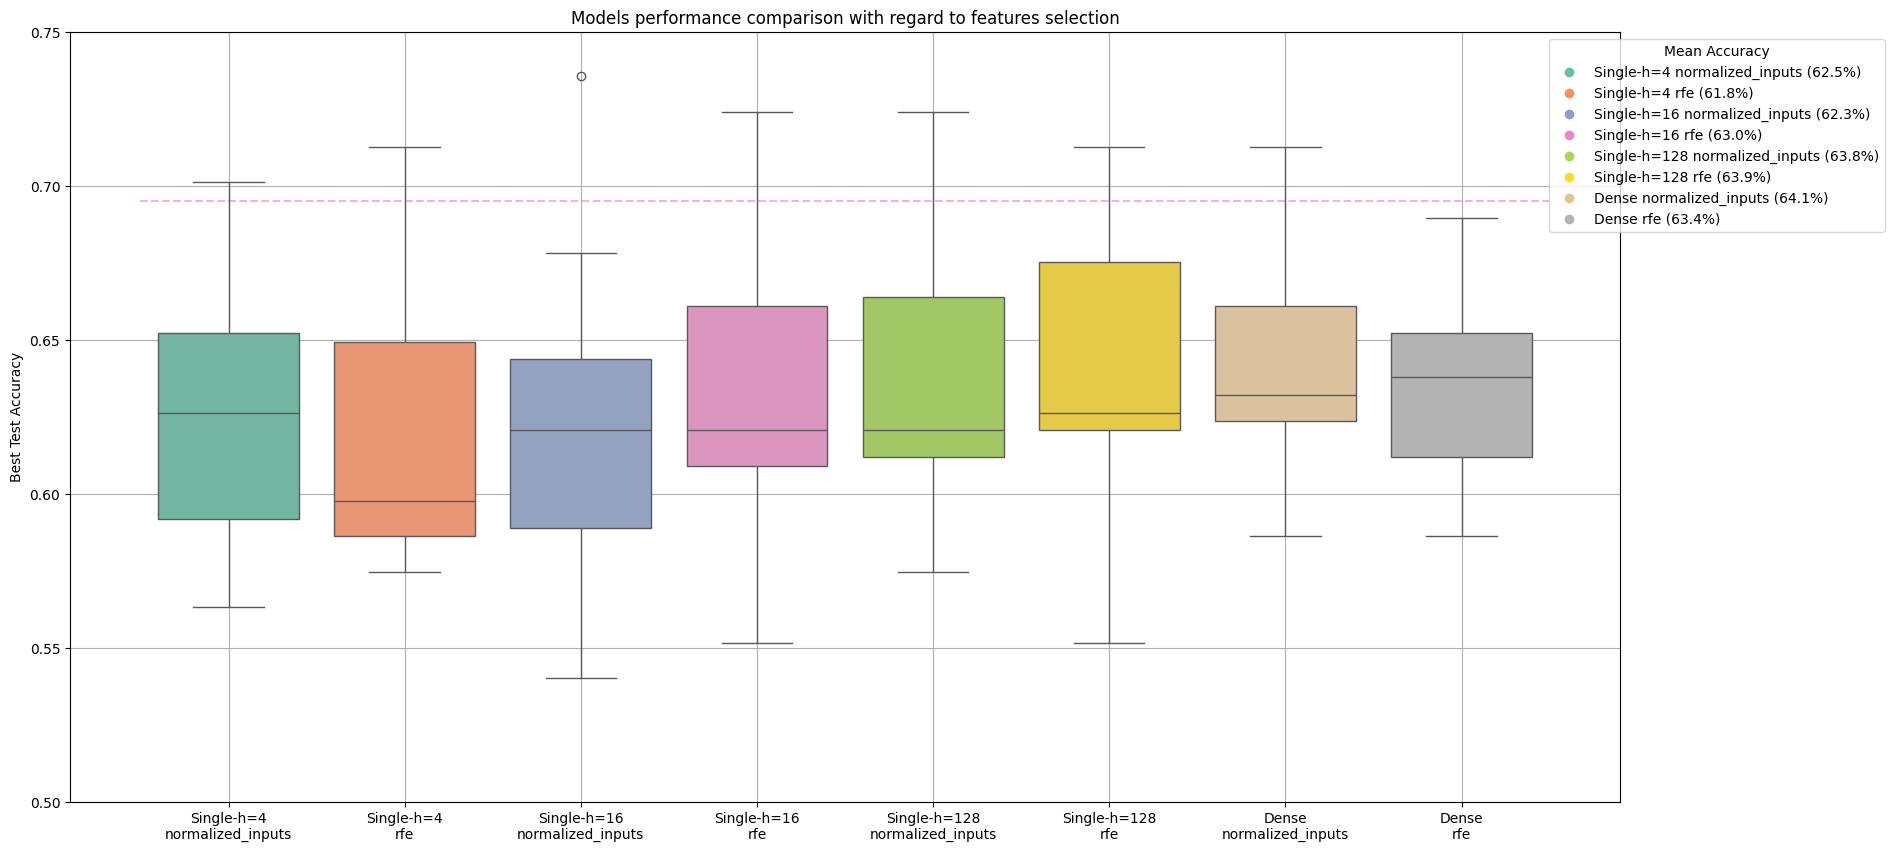
\includegraphics[width=0.5\textwidth]{figures/performances_fully_connected_RFE.png}
    \caption{No significant differences in performance between using all features and using a subset of 2000 features selected with RFE, no matter the number of neurons in the hidden layer.}
    \Description{}
    \label{fig:results_feature_reduction}
\end{figure}

\begin{table}[h!]
	\begin{center}
        \begin{tabular}{lll}
            Model & Feature & Test accuracy \\
            \hline
            Single-h=4 & normalized inputs & 62.5 +/- 4.2\% \\
            Single-h=4 & rfe & 61.8 +/- 4.4\% \\
            Single-h=4 & ae & 59.8 +/- 8.6\% \\
            Single-h=16 & normalized inputs & 62.3 +/- 5.4\% \\
            Single-h=16 & rfe & 63.0 +/- 5.1\% \\
            Single-h=16 & ae & 60.3 +/- 3.9\% \\
            Single-h=128 & normalized inputs & 63.8 +/- 4.3\% \\
            Single-h=128 & rfe & 63.9 +/- 4.6\% \\
            Single-h=128 & ae & 61.7 +/- 4.8\% \\
            Dense & normalized inputs & 64.1 +/- 3.4\% \\
            Dense & rfe & 63.4 +/- 3.3\% \\
            Dense & ae & 60.7 +/- 4.0\% \\
        \end{tabular}
    \end{center}
    \caption{Models performances with regard to feature extraction method}
    \label{table:dependance_on_feature_extraction_method}
\end{table}

Despite the varied configurations tested, it is notable that these setups did not result in significant differences in performance on the test data. Furthermore, the reduction of features through Recursive Feature Elimination (RFE) did not demonstrate any discernible improvement in performance.
Table \ref{table:dependance_on_feature_extraction_method} summarizes the results of our experiments on feature dimensionality reduction.

\subsection{Effect of using graph convolution}

The boxplot \ref{fig:results_architecture} displays the performance of the various configurations in our study. We observe that the use of graph convolutional layers improves the performance of the model as claime by the authors of the original paper.

\begin{figure}[h!]
    \centering
    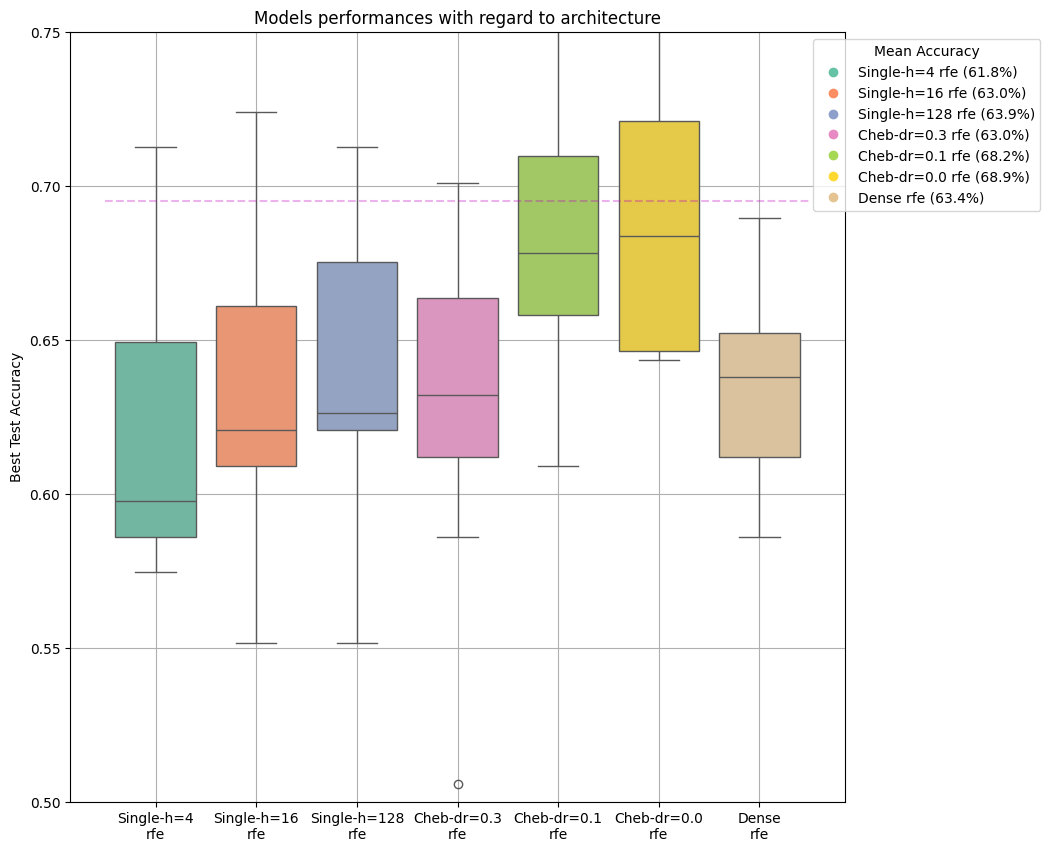
\includegraphics[width=0.45\textwidth]{figures/model_performances_architecture.png}
    \caption{Classification accuracy: comparison of different architectures.
    Single architectures are composed of a single hidden layer with a given number of neurons $h$.
    \textit{Dense} architecture refer to a fully connected neural network with a single hidden layer.
    \textit{Cheb} architectures refer to the graph convolution architecture, we vary the dropout rate $dr$
    during training.}
    \Description{}
    \label{fig:results_architecture}
\end{figure}

\begin{table}[H]
	\begin{center}
		\begin{tabular}{lll}
			Model & Feature & Test accuracy \\
			\hline
			Single-h=4 & rfe & 61.8 +/- 4.4\% \\
			Single-h=16 & rfe & 63.0 +/- 5.1\% \\
			Single-h=128 & rfe & 63.9 +/- 4.6\% \\
			Cheb-dr=0.3 & rfe & 63.0 +/- 5.4\% \\
			Cheb-dr=0.1 & rfe & 68.2 +/- 4.0\% \\
			Cheb-dr=0.0 & rfe & 68.9 +/- 4.0\% \\
			Dense & rfe & 63.4 +/- 3.3\% \\
		\end{tabular}
	\end{center}
	\caption{Models performances with regard to architecture}
	\label{table:dependance_on_architecture}
\end{table}




\subsection{Main limitations}


One prominent challenge that emerged from our experiments was the significant mismatch between the number of subjects ($871$) and the number of features (higher than $6100$), even after dimension reduction techniques were applied. This scenario places us squarely in the realm of the "curse of dimensionality," introducing complexities that can adversely impact the training of neural network models. With a limited number of subjects, the data points within the high-dimensional feature space become sparsely distributed. This sparsity poses challenges for neural networks, as they may struggle to capture meaningful patterns and relationships in the data, leading to overfitting or suboptimal generalization.

In particular, all the models were overfitting the training data, as evidenced by the large gap between the training and validation accuracies. We attempted to mitigate this issue by applying dropout and $L_2$ regularization. We note that the ChebGCN with a dropout rate of $0.1$ yields the best performance on the validation data.

In conclusion, our experiments encompassed a range of configurations, each designed to explore different facets of the model. Despite the diversity in hyperparameters and settings, the performance across these configurations on the test data exhibited minimal variations.